\documentclass{beamer}

\mode<presentation>
{
	\usetheme{CambridgeUS}
	\usecolortheme{orchid}
	\setbeamercovered{transparent}
	\useinnertheme{rectangles}
	\setbeamertemplate{navigation symbols}{}
	\usefonttheme[onlymath]{serif}
	\setbeamercolor{title}{bg=alerted text.fg!85!black, fg=white}
	\setbeamercolor{item projected}{bg=alerted text.fg!85!black}
	\setbeamertemplate{enumerate items}[default]
	\setbeamercolor{local structure}{fg=alerted text.fg!85!black}
}

\usepackage[english]{babel}
\usepackage[utf8]{inputenc}
\usepackage[T1]{fontenc}
\usepackage{lmodern}
\usepackage{underscore}
\usepackage{pifont}


\definecolor{hdblue}{HTML}{3366cc}
\hypersetup{colorlinks,linkcolor=,urlcolor=hdblue, citecolor=hdblue}

\usepackage{amsmath}
\usepackage{outlines}
\usepackage{caption}
\usepackage{subcaption}
\usepackage{bm}
\usepackage{multirow}
\usepackage{natbib}
\usepackage{tikz}

\newcommand{\xmark}{\ding{55}}
\newcommand{\highlight}[1]{%
	\colorbox{red!50}{$\displaystyle#1$}}

\def\ci{\perp\!\!\!\perp}
\makeatletter
\newcommand*{\indep}{%
	\mathbin{%
		\mathpalette{\@indep}{}%
	}%
}


\title[Network and Metagenomics]{Cancer Regulatory Network Modeling and Strain Level Metagenomics Analysis}

% \subtitle
% {Presentation Subtitle} % (optional)

\author[Dogan]
{%
	\texorpdfstring{
		\begin{columns}
			\column{.45\linewidth}
			\centering
			Haluk Dogan\\
			\url{https://haluk.github.io/}\\
			\href{mailto:hdogan@vivaldi.net}{hdogan@vivaldi.net}
		\end{columns}
	}
	{Dogan}
}
\institute[UNL@CSE@SBBI] % (optional, but mostly needed)
{
	Department of Computer Science\\
	University of Nebraska-Lincoln
}

\date[\today] % (optional)
{\today}

\subject{Talks}

\pgfdeclareimage[height=0.5cm]{university-logo}{img/logo}
\logo{\pgfuseimage{university-logo}}

% Delete this, if you do not want the table of contents to pop up at
% the beginning of each subsection:
\AtBeginSubsection[]
{
	\begin{frame}<beamer>{Outline}
		\tableofcontents[currentsection,currentsubsection]
	\end{frame}
}

\begin{document}

\begin{frame}
	\titlepage
\end{frame}

\section{Introduction}
\begin{frame}{Introduction}
	\begin{columns}
		\begin{column}[b]{.48\textwidth}
			Causal modeling of cancer associated genes, miRNAs, and lncRNAs
			\begin{figure}[ht]
				\centering
				\includegraphics[width=1\textwidth]{img/prob.jpeg}
				\caption*{\label{fig:prob} }
			\end{figure}
		\end{column}
		\begin{column}[b]{.48\textwidth}
			Strain level metagenomics analysis
			\begin{figure}[ht]
				\centering
				\includegraphics[width=1\textwidth]{img/metagenome.jpg}
				\caption*{\label{fig:metagenome} }
			\end{figure}
		\end{column}
	\end{columns}
\end{frame}
\begin{frame}{Outline}
	\tableofcontents
\end{frame}

\section{Network Analysis}
\begin{frame}{Network Analysis}
	\begin{figure}[ht]
		\centering
		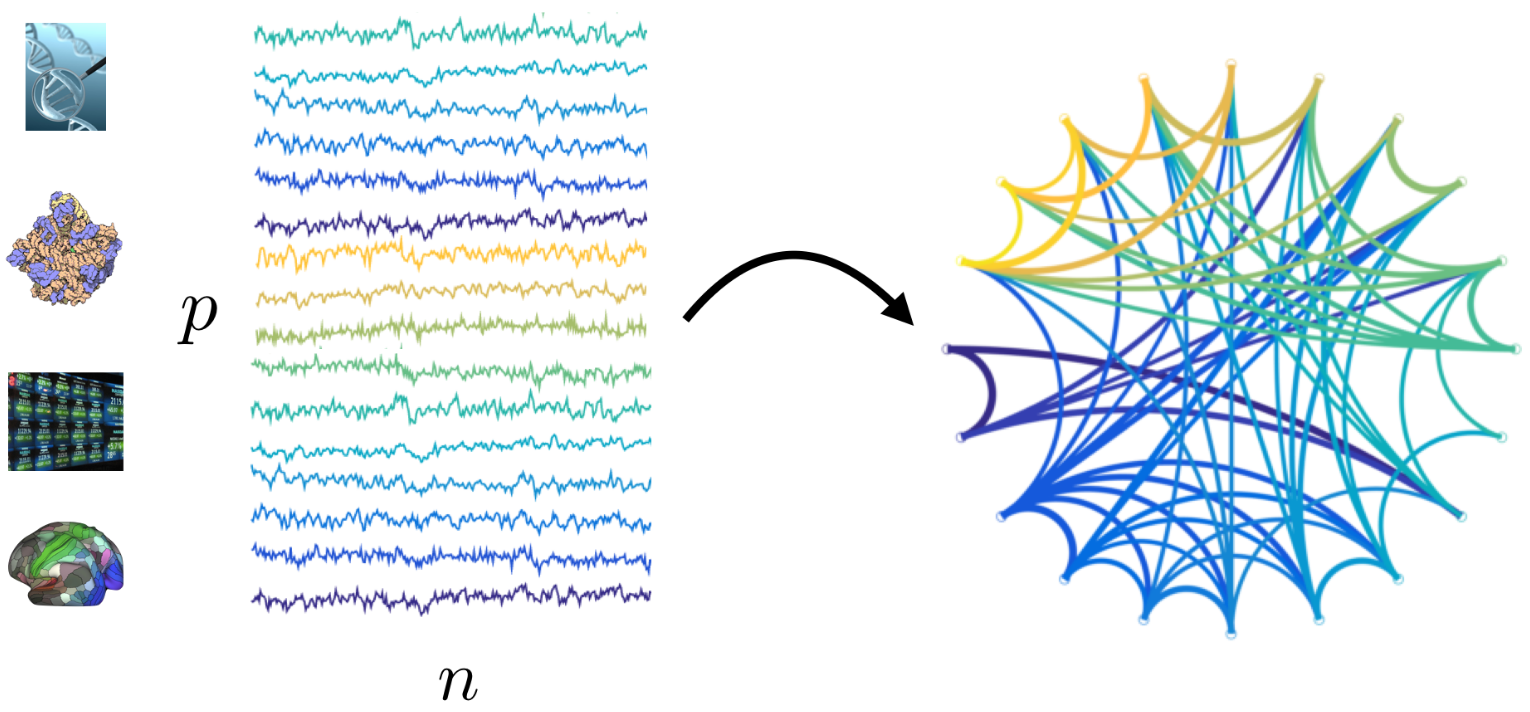
\includegraphics[width=1\textwidth]{img/network.png}
		\caption*{\label{fig:network}}
	\end{figure}
\end{frame}
\begin{frame}{Network Analysis (cont'd)}
	\begin{columns}
		\begin{column}[t]{.48\textwidth}
			Correlation network:
			\begin{figure}[ht]
				\centering
				\includegraphics[width=0.5\textwidth]{img/correlation.png}
				\caption*{\label{fig:correlation-network}}
			\end{figure}
			\vspace{-1.5cm}
			\begin{figure}[ht]
				\centering
				\includegraphics[width=1\textwidth,height=0.4\textheight]{img/correlation-causation.png}
				\caption*{\label{fig:correlation-causation}}
			\end{figure}
		\end{column}
		\begin{column}[t]{.48\textwidth}
			Occam's razor:
			\begin{figure}[ht]
				\centering
				\includegraphics[width=1\textwidth,height=0.7\textheight]{img/elephant.jpg}
				\caption*{\label{fig:elephant}}
			\end{figure}
		\end{column}
	\end{columns}
\end{frame}
\begin{frame}{Gaussian Graphical Models}
	Gene regulatory network:
	\begin{itemize}
		\item $\bm{X}=\left[X_{1}, X_{2}, \dots, X_{p}\right]$
		\item $\bm{X} \sim N(\bm{\mu}, \bm{\Sigma})$
		\item $P(\bm{X} ; \bm{\mu}, \bm{\Sigma})=\frac{1}{(2 \pi)^{p / 2}|\bm{\Sigma}|^{1 / 2}} \exp \left(-\frac{1}{2}(\bm{X}-\bm{\mu})^{T} \bm{\Sigma}^{-1}(\bm{X}-\bm{\mu})\right)$
		\item $\bm{\mu} \in \mathbb{R}^{p}, \boldsymbol{\Sigma} \in \mathbb{S}_{++}^{p}$
		\item Precision matrix: $\bm{\Theta} = \bm{\Sigma}^{-1}$
		\item Challenging problem when $n \ll p$\\
		      Assumptions:
		      \begin{itemize}
			      \item $\bm{\Theta}$ is sparse ($\ell_{1}$)
			      \item Models for each group should not be too different ($\ell_{2}$)
		      \end{itemize}
		\item $\text{Smoke} \ci \text{Heat} \mid \text{Fire}$
	\end{itemize}
\end{frame}
\begin{frame}{Data Augmentation}
	\begin{columns}
		\begin{column}{.48\textwidth}
			Conducting experiments:
			\begin{itemize}
				\item Unethical
				\item Expensive
				\item Difficult to repeat
			\end{itemize}
			\vspace{1cm}
			We used deep learning to generate more in-vitro samples:
			\begin{itemize}
				\item number of samples in groups is imbalanced
				\item unbiased estimator for a learner
			\end{itemize}
		\end{column}
		\begin{column}{.48\textwidth}
			\begin{figure}[ht]
				\centering
				\includegraphics[width=1\textwidth,height=0.7\textheight]{img/deep-learning-image.jpg}
				\caption*{\label{fig:deep-learning}}
			\end{figure}
		\end{column}
	\end{columns}
\end{frame}
\begin{frame}{MiRNA Co-Binding Network}
	\begin{columns}
		\begin{column}[t]{.48\textwidth}
			\begin{figure}[ht]
				\centering
				\includegraphics[width=1\textwidth]{img/mirna-cobinding.jpg}
				\caption*{\label{fig:mirna-cobinding}}
			\end{figure}
			\vspace{-1.5cm}
			\begin{figure}[ht]
				\centering
				\includegraphics[width=1\textwidth]{img/directed.png}
				\caption*{\label{fig:directed}}
			\end{figure}
		\end{column}

		\begin{column}[t]{.48\textwidth}
			\begin{itemize}
				\item We constructed a Bayesian network to represent miRNA co-binding relationships
				\item Evidence matrix is from starBase
				      \begin{table}[]
					      \scalebox{0.7}{
						      \begin{tabular}{|c|l|l|l|l|}
							      \hline
							                  & Gene$_{1}$                                       & Gene$_{2}$ & $\dots$ & Gene$_{n}$ \\ \hline
							      miRNA$_{1}$ & \multicolumn{4}{c|}{\multirow{4}{*}{\huge{1/0}}}                                     \\ \cline{1-1}
							      miRNA$_{2}$ & \multicolumn{4}{l|}{}                                                                \\ \cline{1-1}
							      $\vdots$    & \multicolumn{4}{l|}{}                                                                \\ \cline{1-1}
							      miRNA$_{p}$ & \multicolumn{4}{l|}{}                                                                \\ \hline
						      \end{tabular}
						      \label{table:evidence-matrix}
					      }
				      \end{table}
				\item Intervention to a model is a lot easier
			\end{itemize}
		\end{column}
	\end{columns}
\end{frame}
\begin{frame}{Connecting Models}
	\begin{itemize}
		\item We test each miRNA and dependencies to see if they make significant group difference
		\item We used probabilistic distance metric to measure the data similarity with and without testing miRNAs and their dependencies
		      \begin{itemize}
			      \item Entropic Gromov Wasserstein
		      \end{itemize}
	\end{itemize}
	\begin{columns}
		\begin{column}{.48\textwidth}
			\begin{figure}[ht]
				\centering
				\includegraphics[width=0.7\textheight]{img/earth-mover-distance.jpeg}
				\caption*{\label{fig:emd}}
			\end{figure}
		\end{column}
		\begin{column}{.48\textwidth}
			\begin{figure}[ht]
				\centering
				\includegraphics[width=0.7\textheight]{img/connect-networks.png}
				\caption*{\label{fig:connect-networks}}
			\end{figure}
		\end{column}
	\end{columns}
\end{frame}
\begin{frame}{Data}
	\begin{columns}
		\begin{column}{.48\textwidth}
			\begin{itemize}
				\item Data: TCGA-BRCA
				\item Samples:
				      \begin{itemize}
					      \item Normal: 104
					      \item Stage 1: 179
					      \item Stage 2: 608
					      \item Stage 3: 242
					      \item Stage 4: 20
				      \end{itemize}
				\item DEGs (fold-change $> 2$):
				      \begin{itemize}
					      \item Up: 1218
					      \item Down: 1236
				      \end{itemize}
				\item 617 miRNAs
				      \begin{itemize}
					      \item 1,678 co-binding relationships
					      \item 20,441/166,669 bindings make significant group difference
				      \end{itemize}
			\end{itemize}
		\end{column}

		\begin{column}{.48\textwidth}
			\begin{figure}[ht]
				\centering
				\includegraphics[width=1\textwidth, height=0.7\textheight]{img/diff-genes-volcano.png}
				\caption*{\label{fig:volcano}}
			\end{figure}
		\end{column}
	\end{columns}
\end{frame}
\begin{frame}{Results}
	\begin{columns}
		\begin{column}{.48\textwidth}
			\begin{figure}[ht]
				\centering
				\includegraphics[width=1\textwidth]{img/original-data-heatmap.png}
				\caption*{\label{fig:original-heatmap}}
			\end{figure}
		\end{column}
		\begin{column}{.48\textwidth}
			\begin{figure}[ht]
				\centering
				\includegraphics[width=1\textwidth]{img/data-aug.png}
				\caption*{\label{fig:data-aug}}
			\end{figure}
		\end{column}
	\end{columns}
\end{frame}
\begin{frame}{Results (cont'd)}
	\begin{figure}[ht]
		\centering
		\includegraphics[width=0.7\textwidth,keepaspectratio]{img/network-venn.png}
		\caption*{\label{fig:network-venn}}
	\end{figure}
\end{frame}
\begin{frame}{Results (cont'd)}
	\begin{columns}
		\begin{column}{.48\textwidth}
			\begin{figure}[ht]
				\centering
				\includegraphics[width=1\textwidth]{img/stage1.png}
				\caption{Stage 1\label{fig:stage1}}
			\end{figure}
		\end{column}
		\begin{column}{.48\textwidth}
			\begin{figure}[ht]
				\centering
				\includegraphics[width=1\textwidth]{img/stage2.png}
				\caption{Stage 2\label{fig:stage2}}
			\end{figure}
		\end{column}
	\end{columns}
\end{frame}
\begin{frame}{Results (cont'd)}
	\begin{columns}
		\begin{column}{.48\textwidth}
			\begin{figure}[ht]
				\centering
				\includegraphics[width=1\textwidth]{img/stage3.png}
				\caption{Stage 3\label{fig:stage3}}
			\end{figure}
		\end{column}
		\begin{column}{.48\textwidth}
			\begin{figure}[ht]
				\centering
				\includegraphics[width=1\textwidth]{img/stage4.png}
				\caption{Stage 4\label{fig:stage4}}
			\end{figure}
		\end{column}
	\end{columns}
\end{frame}
\begin{frame}{Results (cont'd)}
	Activated signalling pathways:
	\begin{columns}
		\begin{column}[t]{.48\textwidth}
			\begin{itemize}
				\item Amphetamine addiction
				\item Bacterial invasion of epithelial cells
				\item Chemokine signaling pathway
				\item Complement and coagulation cascades
				\item Cytokine-cytokine receptor interaction
				\item Dilated cardiomyopathy
				\item ECM-receptor interaction
				\item Fanconi anemia pathway
			\end{itemize}
		\end{column}
		\begin{column}[t]{.48\textwidth}
			\begin{itemize}
				\item Focal adhesion
				\item HTLV-I infection
				\item Insulin signaling pathway
				\item Oocyte meiosis
				\item p53 signaling pathway
				\item Salmonella infection
				\item Serotonergic synapse
			\end{itemize}
		\end{column}
	\end{columns}
\end{frame}
\begin{frame}{Results (cont'd)}
	Inhibited signalling pathways:
	\begin{columns}
		\begin{column}[t]{.48\textwidth}
			\begin{itemize}
				\item Adipocytokine signaling pathway
				\item Alcoholism
				\item Amoebiasis
				\item Cell cycle
				\item Fc gamma R-mediated phagocytosis
				\item Focal adhesion
				\item HTLV-I infection
				\item Influenza A
			\end{itemize}
		\end{column}
		\begin{column}[t]{.48\textwidth}
			\begin{itemize}
				\item Malaria
				\item Measles
				\item Pancreatic cancer
				\item Pathways in cancer
				\item PPAR signaling pathway
				\item Progesterone-mediated oocyte maturation
				\item Systemic lupus erythematosus
				\item Tight junction
			\end{itemize}
		\end{column}
	\end{columns}
\end{frame}
\begin{frame}{Results (cont'd)}
	Disease Enrichment on lncRNAs:
	\begin{itemize}
		\item DOID:2449 acromegaly and \textbf{GATA3-AS1}
		\item DOID:299 adenocarcinoma and \textbf{PVT1}
		\item DOID:3355 fibrosarcoma, DOID:8791 breast carcinoma in situ, DOID:8719 in situ carcinoma and \textbf{LINC00987}
	\end{itemize}
\end{frame}
\begin{frame}{Results (cont'd)}
	Low degree miRNAs that make group difference:
	\begin{columns}
		\begin{column}[t]{.48\textwidth}
			\begin{itemize}
				\item hsa-miR-129-5p
				\item hsa-miR-140-3p
				\item hsa-miR-146b-5p
				\item hsa-miR-188-5p
				\item hsa-miR-193a-5p
				\item hsa-miR-28
				\item hsa-miR-346
				\item hsa-miR-3605-3p
			\end{itemize}
		\end{column}
		\begin{column}[t]{.48\textwidth}
			\begin{itemize}
				\item hsa-miR-361
				\item hsa-miR-455-5p
				\item hsa-miR-671-3p
				\item hsa-miR-320b
				\item hsa-miR-193a-3p
				\item hsa-miR-326
				\item hsa-miR-330
				\item hsa-miR-501-3p
			\end{itemize}
		\end{column}
	\end{columns}
\end{frame}
\section{Strain Level Metagenomics Analysis}
\begin{frame}{Strain Level Metagenomics Analysis}
	\vspace{-0.85cm}
	\begin{columns}
		\begin{column}[t]{.44\textwidth}
			\begin{itemize}
				\item Genetic content often varies even within a species
				\item PanPhlAn
				      \begin{itemize}
					      \item Identifies which genes are present in the strains from your sample
				      \end{itemize}
				\item StrainPhlAn
				      \begin{itemize}
					      \item Extracts species-specific marker genes from reads
					      \item Aligns the markers against reference genomes
					      \item Phylogenetic relatedness between strains from different samples
				      \end{itemize}
			\end{itemize}
		\end{column}

		\begin{column}[t]{.52\textwidth}
			\begin{figure}[ht]
				\centering
				\includegraphics[width=0.8\textwidth]{img/biology-classification.png}
				\caption*{\label{fig:biology}}
			\end{figure}
			\vspace{-1.6cm}
			\begin{figure}
				\begin{subfigure}[t]{.48\textwidth}
					\includegraphics[width=0.7\textwidth]{img/bad-bacteria.png}
					\caption{E. coli O157:H7}\label{fig:bad-bacteria}
				\end{subfigure}
				\hfill
				\begin{subfigure}[t]{.48\textwidth}
					\includegraphics[width=0.7\textwidth]{img/good-bacteria.png}
					\caption{E. coli Nissle 1917}\label{fig:good-bacteria}
				\end{subfigure}
			\end{figure}
		\end{column}
	\end{columns}
\end{frame}
\begin{frame}{Data}
	Sample reads are from Bovine milk exosomes
	\begin{itemize}
		\item Negative group:
		      \begin{itemize}
			      \item 3 samples
			      \item ERS, exosome/RNA-sufficient: minimal essential media supplemented with the equivalent of exosomes from 0.5 L bovine milk distributed in the total intestinal water space in an adult, normalized for mice
		      \end{itemize}
		\item Positive group:
		      \begin{itemize}
			      \item 3 samples
			      \item ERD, exosome/RNA-depleted: no exosomes added
		      \end{itemize}
	\end{itemize}
\end{frame}
\begin{frame}{Results}
	\begin{columns}
		\footnotesize{
			\begin{column}[t]{.66\textwidth}
				Identified species from reads:
				\begin{enumerate}
					\item s\textunderscore\@\textunderscore\@Aneurinibacillus\textunderscore\@aneurinilyticus
					\item s\textunderscore\@\textunderscore\@Anaerotruncus\textunderscore\@sp\textunderscore\@G3\textunderscore\@2012
					\item s\textunderscore\@\textunderscore\@Bacillus\textunderscore\@cereus\textunderscore\@thuringiensis
					\item \textbf{s\textunderscore\@\textunderscore\@Clostridium\textunderscore\@sporogenes}
					\item s\textunderscore\@\textunderscore\@Desulfotomaculum\textunderscore\@ruminis
					\item \textbf{s\textunderscore\@\textunderscore\@Enterobacteria\textunderscore\@phage\textunderscore\@lambda}
					\item s\textunderscore\@\textunderscore\@Enterobacteria\textunderscore\@phage\textunderscore\@phiX174\textunderscore\@sensu\textunderscore\@lato
					\item \textbf{s\textunderscore\@\textunderscore\@Enterococcus\textunderscore\@faecalis}
					\item s\textunderscore\@\textunderscore\@Human\textunderscore\@endogenous\textunderscore\@retrovirus\textunderscore\@K
					\item \textbf{s\textunderscore\@\textunderscore\@Lactobacillus\textunderscore\@johnsonii}
					\item s\textunderscore\@\textunderscore\@Oscillibacter\textunderscore\@sp\textunderscore\@1\textunderscore\@3
					\item s\textunderscore\@\textunderscore\@Saccharomyces\textunderscore\@cerevisiae\textunderscore\@killer\textunderscore\@virus\textunderscore\@M1
				\end{enumerate}
			\end{column}
		}
		\begin{column}[t]{.36\textwidth}
			\small{
				\begin{figure}
					\scalebox{0.75}{\input{img/mutation.tikz}}
				\end{figure}
			}
		\end{column}
	\end{columns}
\end{frame}
\begin{frame}{Results (cont'd)}
	\begin{columns}
		\footnotesize{
			\begin{column}{.58\textwidth}
				s\textunderscore\@\textunderscore\@Clostridium\textunderscore\@sporogenes
				\begin{itemize}
					\item 110: 38/38 are in coding region
					\item 101: 459/461 are in coding region (*)
					\item 011: 3279/3292 are in coding region (*)
					\item 001: 44/45 are in coding region (*)
					\item 010: 502/505 are in coding region (*)
				\end{itemize}
			\end{column}
		}
		\begin{column}{.48\textwidth}
			\begin{figure}[ht]
				\centering
				\includegraphics[width=1\textwidth]{img/Clostridium-sporogenes-venn.png}
				\caption*{\label{fig:Clostridium-venn}}
			\end{figure}
		\end{column}
	\end{columns}
\end{frame}
\begin{frame}{Results (cont'd)}
	\begin{figure}[ht]
		\centering
		\includegraphics[width=0.8\textwidth,height=0.3\textheight]{img/Clostridium-sporogenes.png}
		\caption*{\label{fig:Clostridium-hist}}
	\end{figure}
	\vspace{-1cm}
	\begin{figure}[ht]
		\centering
		\includegraphics[width=0.8\textwidth,height=0.4\textheight]{img/Clostridium-sporogenes-msa.png}
		\caption*{\label{fig:Clostridium-msa}}
	\end{figure}
\end{frame}

\begin{frame}{Results (cont'd)}
	\begin{columns}
		\footnotesize{
			\begin{column}{.58\textwidth}
				s\textunderscore\@\textunderscore\@Enterobacteria\textunderscore\@phage\textunderscore\@lambda
				\begin{itemize}
					\item 110: 2/2 are in coding region
					\item 101: 0/0 are in coding region
					\item 011: 1/1 are in coding region
					\item 001: 2/2 are in coding region
					\item 010: 0/0 are in coding region
				\end{itemize}
			\end{column}
		}
		\begin{column}{.48\textwidth}
			\begin{figure}[ht]
				\centering
				\includegraphics[width=1\textwidth]{img/Enterobacteria-phage-lambda-venn.png}
				\caption*{\label{fig:Enterobacteria-venn}}
			\end{figure}
		\end{column}
	\end{columns}
\end{frame}
\begin{frame}{Results (cont'd)}
	\begin{figure}[ht]
		\centering
		\includegraphics[width=0.8\textwidth,height=0.3\textheight]{img/Enterobacteria-phage-lambda.png}
		\caption*{\label{fig:Enterobacteria-hist}}
	\end{figure}
	\vspace{-1cm}
	\begin{figure}[ht]
		\centering
		\includegraphics[width=0.8\textwidth,height=0.4\textheight]{img/Enterobacteria-phage-lambda-msa.png}
		\caption*{\label{fig:Enterobacteria-msa}}
	\end{figure}

\end{frame}

\begin{frame}{Results (cont'd)}
	\begin{columns}
		\footnotesize{
			\begin{column}{.58\textwidth}
				s\textunderscore\@\textunderscore\@Enterococcus\textunderscore\@faecalis
				\begin{itemize}
					\item 110: 1/1 are in coding region
					\item 101: 41/41 are in coding region
					\item 011: 929/929 are in coding region
					\item 001: 1/1 are in coding region
					\item 010: 41/41 are in coding region
				\end{itemize}
			\end{column}
		}
		\begin{column}{.48\textwidth}
			\begin{figure}[ht]
				\centering
				\includegraphics[width=1\textwidth]{img/Enterococcus-faecalis-venn.png}
				\caption*{\label{fig:Enterococcus-venn}}
			\end{figure}
		\end{column}
	\end{columns}
\end{frame}
\begin{frame}{Results (cont'd)}
	\begin{figure}[ht]
		\centering
		\includegraphics[width=0.8\textwidth,height=0.3\textheight]{img/Enterococcus-faecalis.png}
		\caption*{\label{fig:Enterococcus-hist}}
	\end{figure}
	\vspace{-1cm}
	\begin{figure}[ht]
		\centering
		\includegraphics[width=0.8\textwidth,height=0.4\textheight]{img/Enterococcus-faecalis-msa.png}
		\caption*{\label{fig:Enterococcus-msa}}
	\end{figure}

\end{frame}

\begin{frame}{Results (cont'd)}
	\begin{columns}
		\footnotesize{
			\begin{column}{.58\textwidth}
				s\textunderscore\@\textunderscore\@Lactobacillus\textunderscore\@johnsonii
				\begin{itemize}
					\item 110: 39/39 are in coding region
					\item 101: 17/17 are in coding region
					\item 011: 1113/1119 are in coding region (*)
					\item 001: 42/42 are in coding region
					\item 010: 18/18 are in coding region
				\end{itemize}
			\end{column}
		}
		\begin{column}{.48\textwidth}
			\begin{figure}[ht]
				\centering
				\includegraphics[width=1\textwidth]{img/Lactobacillus-johnsonii-venn.png}
				\caption*{\label{fig:Lactobacillus-venn}}
			\end{figure}
		\end{column}
	\end{columns}
\end{frame}
\begin{frame}{Results (cont'd)}
	\begin{figure}[ht]
		\centering
		\includegraphics[width=0.8\textwidth,height=0.3\textheight]{img/Lactobacillus-johnsonii.png}
		\caption*{\label{fig:Lactobacillus-hist}}
	\end{figure}
	\vspace{-1cm}
	\begin{figure}[ht]
		\centering
		\includegraphics[width=0.8\textwidth,height=0.4\textheight]{img/Lactobacillus-johnsonii-msa.png}
		\caption*{\label{fig:Lactobacillus-msa}}
	\end{figure}

\end{frame}


\section{Conclusion}
\begin{frame}{Questions}
	\begin{center}
		\Huge{Questions?}
	\end{center}
	\begin{figure}
		\centering
		\includegraphics[width=0.5\textwidth, height=1.0\textheight, keepaspectratio]{img/walter.jpg}
	\end{figure}
\end{frame}
\end{document}

%%% Local Variables:
%%% mode: latex
%%% TeX-master: t
%%% End:
